\section{Sicherheitsaspekte der Android-Architektur}

	Bereits durch die Architektur des Betriebssystems, insbesondere durch die restriktive Rechtevergabe und das Sandboxing, wird versucht, ein möglichst sicheres System bereitzustellen. Ab Android Version 4.3 kommt zusätzlich noch \textit{Security-Enhanced Linux (SELinux)} zum Einsatz.\\
	Verschlüsselungen und Signaturen werden Hardwareseitig durch eine \textit{Trusted Execution Environment (TEE)} unterstützt. TEE stellt einen besonders geschützten Bereich auf dem Prozessor dar, auf dem nur berechtige Anwendungen ausgeführt werden können. Die Implementierung ist dabei Prozessor Hersteller abhängig - auf ARM wird dabei, wie bei iOS, auf \textit{TrustZone}\cite{TEE_ARM} zurückgegriffen.
	
	\subsection{Verified Boot}
	Bereits während des Bootvorgangs muss die Sicherheit und Integrität des Bootmediums sichergestellt werden. Dadurch kann eine Veränderung, z.B. durch eine Infektion, frühzeitig erkannt werden.\\
	Der Integritätscheck basiert auf der Kernelfunktion \textit{dm-verity} welche einen Hash-Tree, unter Nutzung von SHA-256, aufbaut. Dabei werden von jedem 4K Sektor ein Hash berechnet und je zwei Hashes zu einem gehasht. Diese Operation wird solange wiederholt bis nur noch ein einziger Wert übrige ist - der \textit{root hash}.
	\begin{figure}[h]
	\centering
	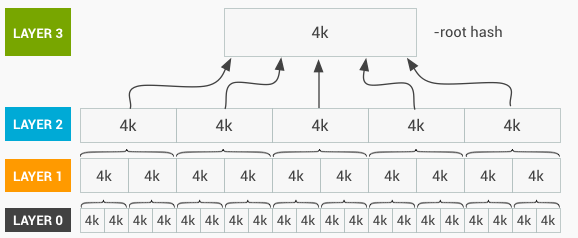
\includegraphics[width=0.7\linewidth]{android_pages/graphics/dm-verity-table}
	\caption[Aufbau des Hash-Trees]{Aufbau des von dm-verity erstellten Hash-Trees\protect\cite{VerifiedBoot}}
	\label{fig:dm-verity-table}
	\end{figure}
	Da allerdings diese Überprüfung vom Kernel übernommen wird, muss auch die Integrität des Kernels und Bootloaders überprüft werden. Die geschieht mittels einer Signatur und eines, in Hardware festgeschriebenen, OEM Keys. Sollte dieser Test nicht erfolgreich sein, wird die Partition über ein Zertifikat, welches in der Paritions Signatur zu finden ist, verifiziert. Diese Variante wird auch genutzt, um inoffizielle Images zu verifizieren. \\
	Um grundsätzlich zwischen einem Gerät mit offiziellen und inoffiziellen Image zu unterscheiden, gibt es zwei Status: \textit{LOCKED} und \textit{UNLOCKED}
%	\begin{quote}
	%	\begin{itemize}\itemsep0pt
		%	\item GREEN, indicating a full chain of trust extending from the bootloader to verified partitions, including the %bootloader, boot partition, and all verified partitions. 
		%	\item YELLOW, indicating the boot partition has been verified using the embedded certificate, and the signature is %valid. The bootloader is required to display a notification and the fingerprint of the public key during boot.
		%	\item ORANGE, indicating a device may be freely modified. Device integrity is left to the user to verify %out-of-band. The bootloader must display a warning to the user before allowing the boot process to continue. 
		%	\item RED, indicating the device has failed verification. The bootloader must display a warning to the user before %allowing the boot process to continue. 
	%	\end{itemize}
	%	\cite{VerifyingBoot}
	%\end{quote}
	%Da ersteres Vorgehen nur bei offiziellen Boot Images möglich ist, wurden zusätzlich noch zwei grundlegende Status mit %eingebaut. \textit{LOCKED} und \textit{UNLOCKED};  über diese Status wird angegeben ob gegen einen OEM Key geprüft %(LOCKED) werden soll oder nicht (UNLOCKED). Damit ist es möglich eigene Boot Images zu nutzen. Es kommt lediglich beim %Hochfahren des Systems eine Meldung.
	Der komplette Ablauf ist in der nachfolgenden Grafik nochmal übersichtlich dargestellt.
	\begin{figure}[h]
		\centering
		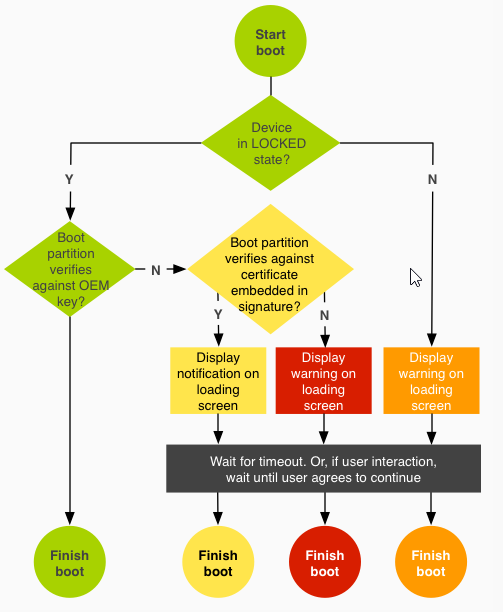
\includegraphics[width=0.6\linewidth, height=0.4\textheight]{android_pages/graphics/VerifiedBoot}
		\caption[Verified boot flow\protect\cite{VerifyingBoot}]{Verified boot flow\protect\cite{VerifyingBoot}}
		\label{fig:VerifiedBoot}
	\end{figure}

\begin{flushleft}
	Zu beachten ist allerdings, dass dieses Feature erst mit Android 4.4 eingeführt wurde. In Älteren Versionen gibt es keinerlei derartigen Check.
\end{flushleft}


	\subsection{Basis Rechtesystem}\label{sec:BasisRechteSystem}
	Von Linux wurde auch das Basis-Rechtesystem "ubernommen. Hierbei bekommt jede App eine eindeutige User-ID (UID) zugewiesen, welche im Normalfall zur Installationszeit zugeteilt wird. Jeder Nutzer, und somit auch jede App, arbeitet grundsätzlich erst einmal nur innerhalb der ihm zugewiesenen virtuellen Maschine und dem damit verbundenen Dateisystem.\\\\
	Da es dennoch in vielen Fällen nötig ist, Daten zwischen verschiedenen Apps auszutauschen, gibt es mehrer Möglichkeiten dies zu tun. Die üblichen Wege wären Intends oder SharedPreferences. Zusätzlich gibt es noch die Möglichkeit mehreren Apps dieselbe UID zuweisen zu lassen. Dies ist allerdings nur möglich, wenn die entsprechenden Applikationen mit dem selben Zertifikat signiert wurden und in deren Manifest Datei eine gemeinsame UID festgelegt wurde.
	Durch dieses Rechtesystem wird versucht sicherzustellen, dass kein Nutzerprogramm als \textit{root} ausgeführt wird.
	
	\subsection{Sandboxing und Permissions} \label{sec:SandBoxingNPermissions}
	Wie bereits erwähnt, laufen die Applikationen jeweils in ihrer eigenen Sandbox. Grundsätzlich ist die App damit in ihrer Ausführung auf ihren Bereich beschränkt und kann nicht mit anderen Prozessen und Daten ausserhalb interagieren. Dennoch ist es in den meisten Fällen sinnvoll mit Systemservices und Nutzerdaten zu interagieren, die nicht in der eigenen Sandbox verfügbar sind. 
	
	\subsubsection{Permissions im Detail}
	Um nun die bestehenden Zugriffsrechte erweitern zu können, müssen die entsprechenden Rechte (Permissions) in der Manifest Datei deklariert und angefordert werden. Zu Installationszeit werden diese Permissions dem Nutzer angezeigt und dieser wird gefragt, ob er den Rechtswünschen der App zustimmt oder nicht. Dabei gilt das \textit{Alles-Oder-Nichts-Prinzip}, d.h. entweder bekommt die Anwendung alle Rechte oder keine - was eine nicht Installation zur Folge hat. Des weiteren können die Berechtigungen nach der Installation nicht mehr angepasst werden.\\
	Oben genannte Berechtigungen sind beispielsweiße für Zugriffe auf externe Speichermedien oder auch die Kamera nötig. Dabei ist allerdings zu beachten, dass die Permissions zum Teil sehr grob definiert sind. Wodurch für den Nutzer nicht unbedingt erkenntlich ist, welche Informationen eine App warum abgreift und ob die App wirklich Gebrauch des Rechts macht.\\
	Anhand der folgenden Permission lässt sich die daraus resultierende Problematik gut erkennen:\\
	RECORD\_AUDIO Permission:
	\begin{quote}
	Allows an application to record audio \footnote{https://developer.android.com/reference/android/Manifest.permission.html\#RECORD\_AUDIO}
	\end{quote} 
	Dabei ist für den Nutzer nicht sichtbar, wann eine Aufnahme läuft, ausser die Applikation stellt dafür einen Hinweis bereit - wobei hier die Frage ist ob dieser auch wirklich verlässlich ist. Stellt die App einen Service bereit, kann ein solcher Mitschnitt auch im Hintergrund geschehen, und damit auch während eines Telefonats. Die einzige Chance RECORD\_AUDIO zur Laufzeit zu unterbinden ist, den Service bzw. die App über den Anwendungsmanager zu beenden.\\
	Dieses Problem ist auf die meisten anderen Berechtigungen übertragbar.\\\\
%	Für die nächste Android Version, Android M, ist eine Verbesserung dieses Berechtigungssystems geplant und auch bereits vorgestellt worden. Es wird nun ermöglicht zur Laufzeit von Applikationen diesen Berechtigungen zu entziehen und freizugeben. Damit bekommt der Nutzer deutlich mehr Möglichkeiten, um seine Daten zu schützen. Allerdings wird es wohl kein Update für ältere Versionen geben, wodurch dort das Problem bestehen bleibt.
	Mit Android 4.3 (Kitkat) wurde eine versteckte Einstellungs-Activity namens \textit{App Ops} eingeführt. Darin konnte man einsehen welche App, wann welche Permission genutzt hat, und dieser einzelne Rechte zu entziehen und wieder zu erlauben. Diese Funktion konnte nur durch das Anlegen eines Activity Shortcuts und der direkten Verwendung in einer App genutzt werden. Leider wurde diese versteckte Einstellung aus den nächsten Versionen entfernt - bis Android M. \cite{HiddenActivity} \\
	Für Android M wurde mittlerweile angekündigt, dass eine derartige Einstellung nun fest mit eingebaut sein wird.
	Allerdings wird es wohl kein Update für ältere Versionen geben, wodurch das Problem in diesen bestehen bleibt.
	
	\subsubsection{Besonderheit: Systemapps}
	Apps des Smartphone Hersteller können Rechte besitzen, die für normale Anwendungen nicht verfügbar sind, um Basis Apps und Services bereit zustellen. Hierfür werden alle Hersteller Applikationen mit sogenannten \textit{Publisher Keys} signiert, dadurch können, wie bereits unter \ref{sec:BasisRechteSystem} erklärt, diese Anwendung bspw. im selben Prozess laufen.
	
	\subsection{SELinx in Android}
	\begin{quote}
	SELinux operates on the ethos of default denial. Anything that is not explicitly allowed is denied.\cite{SELinuxAndroid}
	\end{quote}
	Durch die Nutzung von SELinux soll das vorhandene Berechtigungssystem und Sandboxing unterstützt und verstärkt werden. Dabei sind zwei Nutzungsmodi zu unterscheiden. Während im \textit{permissive mode} Regelverstöße nur geloggt werden, wird im \textit{enforcing mode} die strikte Einhaltung erzwungen. In den Versionen 4.3 bis exklusive 5.0 war der \textit{enforcing mode} nicht überall in Nutzung. Dies änderte sich ab Version 5.0, seit dem läuft nur noch dieser Modus.
	 
	
	

	